\documentclass{mp}
\graphicspath{{10_korelacja}}
\subtitle{Momenty wielowymiarowe}
\DeclareMathOperator{\cov}{cov}
\begin{document}
\frame{\titlepage}
\begin{frame}{Momenty zmiennych losowych}
\begin{block}{Moment rzędu $l$ względem punktu $c$}
\[ E(X-c)^l=\begin{cases} \sum_{x_i} (x_i-c)^lp_i & $X$\text{ typu skokowego} \\
\int_{-\infty}^\infty (x-c)^lf(x)\d{x} & $X$\text{ typu ciągłego}
\end{cases} \]
\end{block}
\begin{description}
\item[moment zwykły] $c=0$
\item[moment centralny] $c=\mu$
\end{description}
\end{frame}
\begin{frame}{Momenty dwuwymiarowe}
\begin{description}
\item<+->[moment zwykły rzędu $l+r$] \[E(X^lY^r)\]
\item<+->[moment centralny rzędu $l+r$] \[E((X-EX)^l(Y-EY)^r)\]
\item<+->[kowariancja] \[\cov(X,Y)=E((X-EX)(Y-EY))=EXY-EXEY\]
\end{description}
\only<+->
{
\begin{block}{Twierdzenie}
\[\left(\forall x,y\in\R\colon P(X<x,Y<y)=P(X<x)P(Y<y) \right) \to cov(X,Y)=0 \]
\end{block}
}
\end{frame}
\begin{frame}{Współczynnik korelacji}
\[\varrho=\frac{\cov(X,Y)}{\sigma_X\sigma_Y} \]
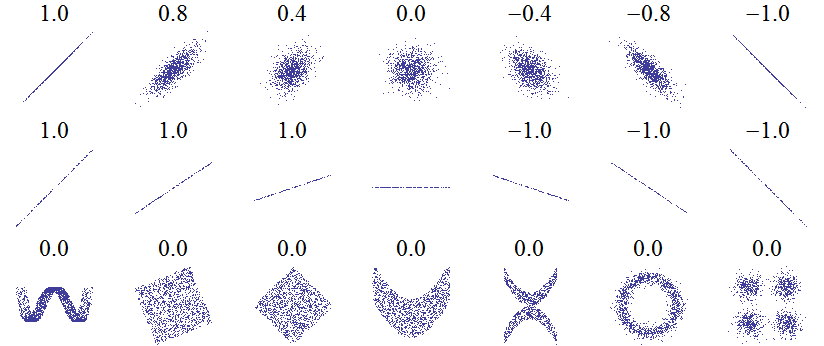
\includegraphics[width=\textwidth]{10_korelacja/Correlation_examples.png}

{\tiny \url{http://upload.wikimedia.org/wikipedia/commons/0/02/Correlation_examples.png} domena publiczna}
\end{frame}
\begin{frame}{Podejrzane korelacje}
\url{http://tylervigen.com/}
\end{frame}

%\item<+->[wektor wartości średnich] \[\mathbf{\mu}=\begin{pmatrix}\mu_{1,0}\\\mu_{0,1}\end{pmatrix}\only<+->{=\begin{pmatrix}\mu_X\\\mu_Y\end{pmatrix}}\]
%\item<+->[macierz kowariancji] \[\Sigma=\begin{bmatrix}\sigma_{2,0} & \sigma_{1,1} \\ \sigma_{1,1} & \sigma_{0,2} \end{bmatrix}\]
\end{document}
